\capitulo{5}{Aspectos relevantes del desarrollo del proyecto}

En este apartado se recogen los detalles con mayor importancia en el desarrollo del proyecto. Tratando de mantener un orden cronológico con el que observemos los pasos que hemos seguido para solucionar las problemáticas del trabajo.

\begin{comment}
Este apartado pretende recoger los aspectos más interesantes del desarrollo del proyecto, comentados por los autores del mismo.
Debe incluir desde la exposición del ciclo de vida utilizado, hasta los detalles de mayor relevancia de las fases de análisis, diseño e implementación.
Se busca que no sea una mera operación de copiar y pegar diagramas y extractos del código fuente, sino que realmente se justifiquen los caminos de solución que se han tomado, especialmente aquellos que no sean triviales.
Puede ser el lugar más adecuado para documentar los aspectos más interesantes del diseño y de la implementación, con un mayor hincapié en aspectos tales como el tipo de arquitectura elegido, los índices de las tablas de la base de datos, normalización y desnormalización, distribución en ficheros3, reglas de negocio dentro de las bases de datos (EDVHV GH GDWRV DFWLYDV), aspectos de desarrollo relacionados con el WWW...
Este apartado, debe convertirse en el resumen de la experiencia práctica del proyecto, y por sí mismo justifica que la memoria se convierta en un documento útil, fuente de referencia para los autores, los tutores y futuros alumnos.
\end{comment}

\section{Procesamiento de imágenes}

Como primera aproximación al problema que nos concierne, nos hemos enfrentado al procesamiento de imágenes mediante la librería \textit{Scikit-image} de \textit{Python}. Mediante esta herramienta trataremos de dar solución a nuestro problema siguiendo los siguientes pasos:

\begin{enumerate}[1.]
  \item Convertir la imagen a escala de grises
  \item Segmentar los objetos del fondo de la imagen
  \item Obtener los distintos objetos de la imagen
\end{enumerate}

\subsection{Convertir la imagen a escala de grises}

La conversión de la imagen original (RGB) a escala de grises viene motivada con el mero objetivo de poder segmentar los objetos del fondo de la imagen mediante el método de \textit{Thresholding}. Solo pudiéndose partir de una imagen en escala de grises. En la figura \ref{fig:5.1.1} podemos ver los resultados.

\begin{figure}
	\centering
	\begin{subfigure}[b]{0.45\textwidth}
        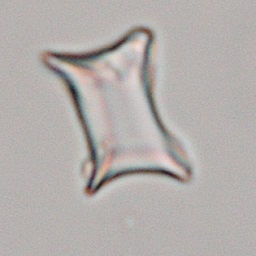
\includegraphics[width=\textwidth]{2}
        \caption{Original}
    \end{subfigure}
    \begin{subfigure}[b]{0.45\textwidth}
        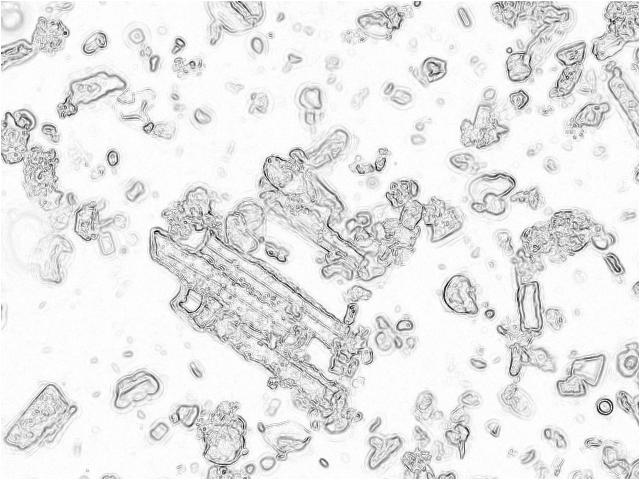
\includegraphics[width=\textwidth]{grayscale_image}
        \caption{Imagen en escala de grises}
    \end{subfigure}
    \caption{Conversión de la imagen original a escala de grises}
	\label{fig:5.1.1}
\end{figure}

\subsection{Segmentar los objetos del fondo de la imagen}

Una vez tenemos la imagen en escala de grises, procedemos a transformar nuestra imagen en una imagen en blanco y negro o binarizada. Los motivos por los que binarizamos la imagen es para obtener una imagen que sea más significativa para nosotros y además este simplificada. Lo cual nos será útil para facilitarnos su procesamiento.

\textit{Scikit-image} nos propociona distintos métodos mediante los cuales podemos segmentar una imagen. En la figura \ref{fig:5.1.2} podemos observar el resultado aplicando distintos métodos, los cuales se van indicando en cada una de las figuras.

\begin{figure}
	\centering
	\begin{subfigure}[b]{0.45\textwidth}
        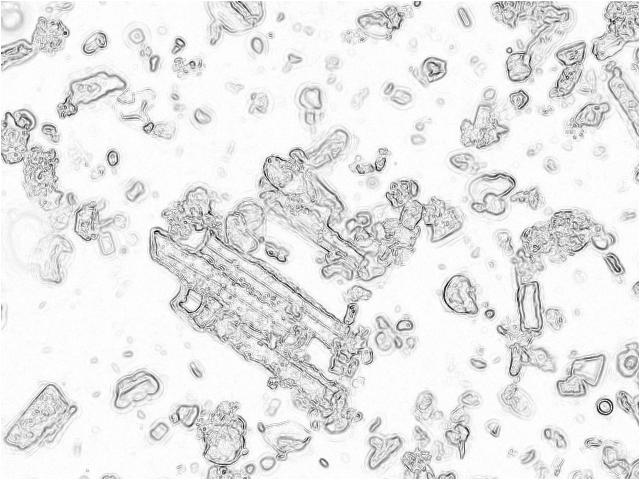
\includegraphics[width=\textwidth]{grayscale_image}
        \caption{Imagen en escala de grises}
    \end{subfigure}
    \begin{subfigure}[b]{0.45\textwidth}
        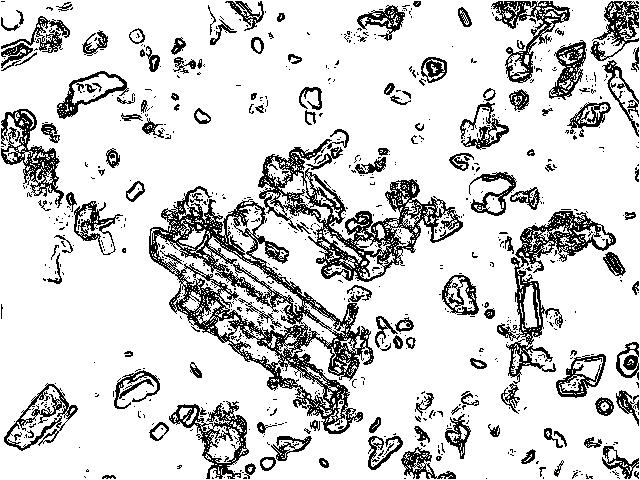
\includegraphics[width=\textwidth]{otsu_threshold_image}
        \caption{Método de Otsu}
    \end{subfigure}
    \begin{subfigure}[b]{0.45\textwidth}
        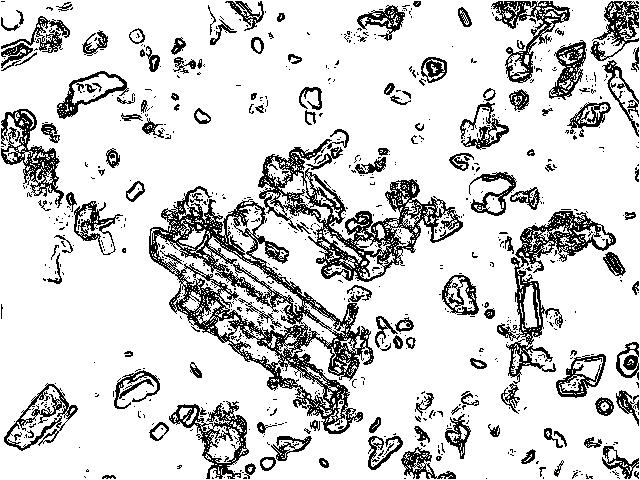
\includegraphics[width=\textwidth]{otsu_threshold_image}
        \caption{Método de Otsu}
    \end{subfigure}
    \begin{subfigure}[b]{0.45\textwidth}
        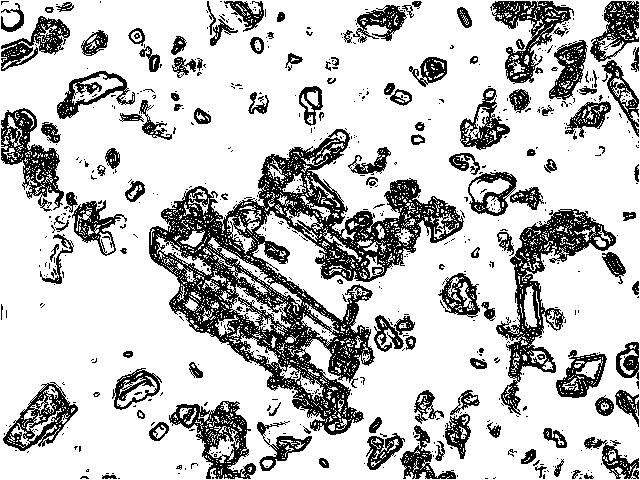
\includegraphics[width=\textwidth]{yen_image}
        \caption{Método de Yen}
    \end{subfigure}
    \begin{subfigure}[b]{0.45\textwidth}
        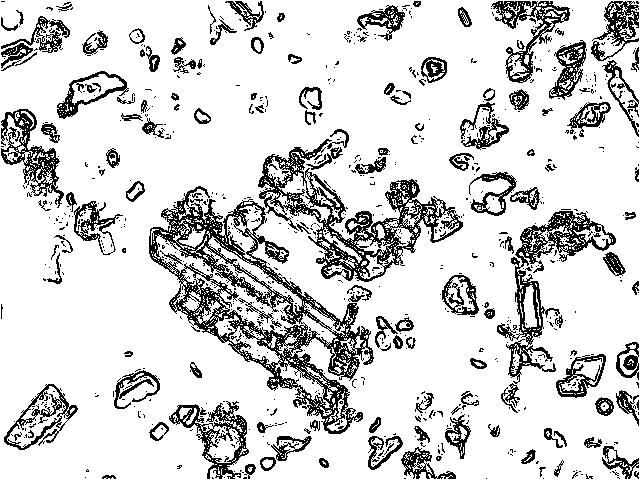
\includegraphics[width=\textwidth]{li_thresholded_image}
        \caption{Método de Li}
    \end{subfigure}
    \begin{subfigure}[b]{0.45\textwidth}
        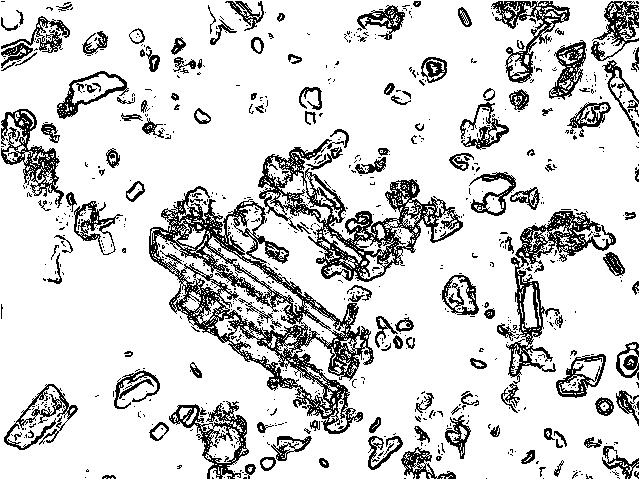
\includegraphics[width=\textwidth]{isodata_thresholded_image}
        \caption{Método de ISODATA}    
    \end{subfigure}
    \begin{subfigure}[b]{0.45\textwidth}
        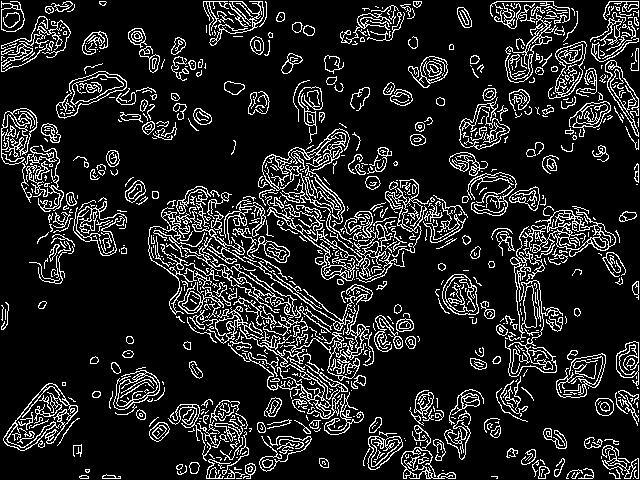
\includegraphics[width=\textwidth]{edge_based_image}
        \caption{Método basado en bordes}    
    \end{subfigure}
    \begin{subfigure}[b]{0.45\textwidth}
        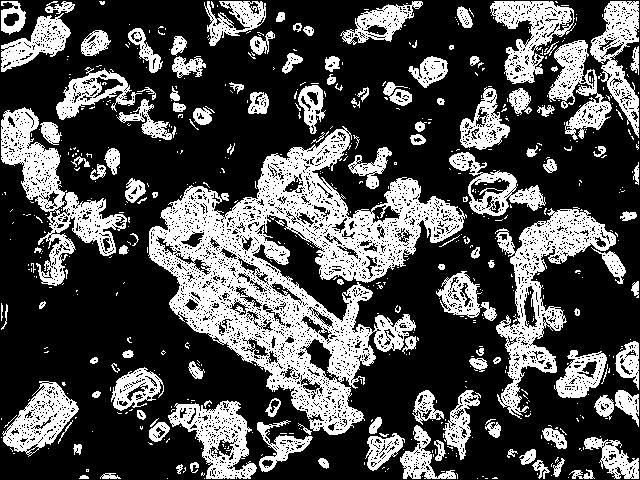
\includegraphics[width=\textwidth]{adaptive_thresholded_image_5}
        \caption{Método adaptativo}    
    \end{subfigure}
    \caption{Distintos ejemplos de una imagen segmentada}
	\label{fig:5.1.2}
\end{figure} 

\subsection{Obtener los distintos objetos de la imagen}
Después de tener la imagen binarizada de la forma más apropiada posible probamos a segmentar los distintos objetos de nuestra imagen.

\subsection{Transformación divisoria}
Transformación divisoria, o en inglés \textit{Watershed segmentation}, es un algoritmo clásico para la segmentación de objetos en una imagen.

Durante las primeras pruebas, la segmentación más interesante hasta el momento ha sido la que se muestra en la figura \ref{fig:5.1.3}. A partir de \textit{Watershed segmentation} con marcado, representando cada color un objeto distinto. Más allá de esta segmentación no se ha conseguido nada mejor.

\begin{figure}
	\centering
	\begin{subfigure}[b]{0.45\textwidth}
        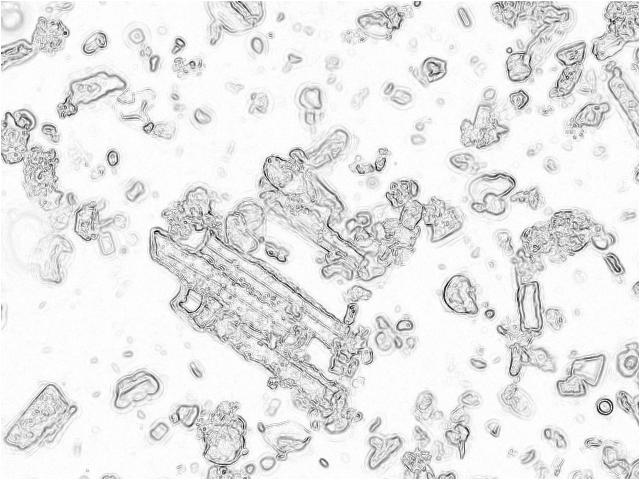
\includegraphics[width=\textwidth]{grayscale_image}
        \caption{Imagen en escala de grises}
    \end{subfigure}
    \begin{subfigure}[b]{0.45\textwidth}
        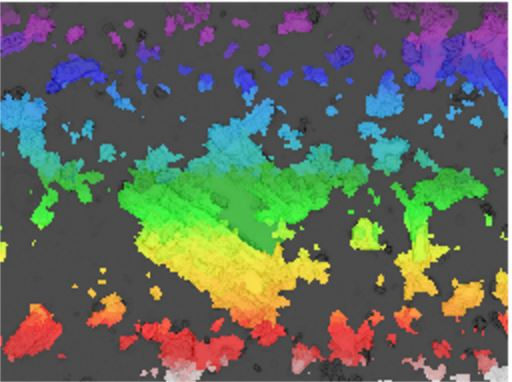
\includegraphics[width=\textwidth]{segmented}
        \caption{Imagen segmentada}
    \end{subfigure}
        \caption{Resultados obtenidos mediante transformación divisoria}
	\label{fig:5.1.3}
\end{figure} 	

\section{Clasificadores}

La aproximación mediante procesamiento de imágenes no parece la más adecuada visto los resultados obtenidos. Por ello vamos a realizar el estudio sobre una segunda aproximación  mediante clasificadores, junto a descriptores visuales y la técnica de la ventana deslizante, o en inglés \textit{sliding window}.

\textit{Sliding window} consiste en la subdivisión de una imagen en distintos fragmentos, estableciendo previamente el tamaño de los fragmentos, tanto en ancho como en alto, y el tamaño del salto en cada eje, tras una subdivisión. 

Como podemos apreciar en la figura \ref{fig:sliding_window}, primero, la ventana deslizante recorre la imagen en el eje horizontal. Comenzando por la esquina superior izquierda hasta llegar a la esquina superior derecha. Generando una imagen por cada subdivisión y realizando saltos horizontales según el tamaño que hayamos definido. Una vez esta llega a la esquina superior derecha, la ventana deslizante lleva a cabo el mismo proceso pero realizando un salto en el eje vertical. Y así sucesivamente hasta completar su recorrido por toda la imagen.

\begin{figure}
\centering
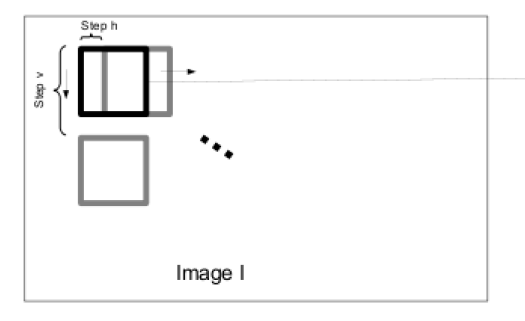
\includegraphics[width=0.8\textwidth]{sliding_window}
\caption{Esquema del funcionamiento de la ventana deslizante}
\label{fig:sliding_window}
\end{figure}

El primer conjunto de técnicas escogidas ha sido una Máquina de Vector Soporte junto al Histograma de los gradientes orientados, la cual es una técnica para la extracción automática de características. Sin embargo, iremos utilizando distintas técnicas para adoptar la que mejor se adapte a nuestra problemática.

El procedimiento para obtener el clasificador es el siguiente:

\begin{enumerate}[1.]
  \item Crear un conjunto de entrenamiento de imágenes de caras que consideramos que son elementos positivos.
  \item Crear un conjunto de entrenamiento de imágenes de no-caras que consideramos que son negativos.
  \item Extraer las características del conjunto de entrenamiento  mediante un descriptor visual.
  \item Entrenar\footnote{Nos referimos por entrenar, en este ámbito, a enviar al clasificador las distintas imágenes con la clase a la que pertenecen (fitolito de tipo 1, fitolito de tipos 2, etc.).} el clasificador.
\end{enumerate}

 Finalizado el entrenamiento, ya tenemos nuestro clasificador listo para enviarle nuevas imágenes y que sean clasificadas.
 
\subsection{Reconocimiento de imágenes en nuevas imágenes}
Para el reconocimiento de objetos en nuevas imágenes, deberemos llevar a cabo los tres siguientes pasos:

\begin{enumerate}[1.]
  \item Dividir la imagen en múltiples fragmentos.
  \item Comprobar si cada uno de los fragmentos contiene el objeto.
  \item Si existe solapamiento en la detección de objetos, muy común en el uso de este tipo de clasificadores, se deben de combinar dichos solapamientos en uno único.
\end{enumerate}

Cada uno de los fragmentos anteriores se solapa en gran medida. Por lo que origina un problema de sobrereconocimiento de objetos, reconociendo donde existe un posible positivo, más de uno, en la mayoría de casos. Por ello, se aplica el tercer paso sobre los objetos reconocidos, que es la eliminación del solapamiento de objetos mediante la técnica de \textit{Non-maximum suppression}.

\subsection{Aplicación sobre el reconocimiento de caras}

Como previa experimentación con esta metodología, vamos a entrenar el clasificador para el reconocimiento de caras. Y en función de la efectividad del método sobre las caras tomaremos una serie de conclusiones sobre las que decidiremos si llevar a cabo esta solución sobre  nuestro problema.

Como explicábamos anteriormente, una vez tenemos nuestro clasificador le enviamos una nueva imagen, como podría ser la presentada en la figura \ref{subfig:family}. A partir de esta imagen el clasificador nos permitirá obtener las ventanas \footnote{Se entiende por ventana, en este contexto, a la caja o cuadrilatero que etiqueta un positivo en una imagen.} en las que detecta una cara, como vemos en la figura \ref{subfig:family_labeled}. Podemos apreciar que existe más de una ventana alrededor de cada cara. Y finalmente, tras aplicar el método \textit{Non-Maximum supresion} obtenemos el resultado final mostrado en la figura \ref{subfig:family_labeled_nms}.

\begin{figure}
	\centering
	\begin{subfigure}[b]{0.45\textwidth}
        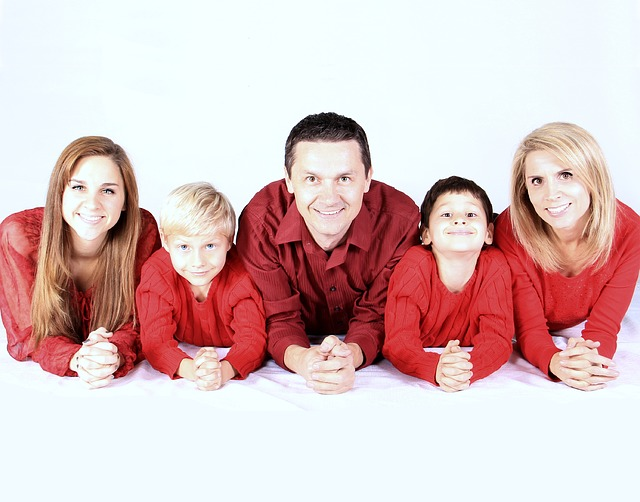
\includegraphics[width=\textwidth]{family}
        \caption{Imagen original}
        \label{subfig:family}
    \end{subfigure}
    \begin{subfigure}[b]{0.45\textwidth}
        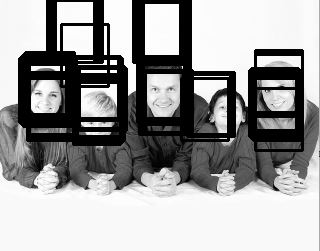
\includegraphics[width=\textwidth]{family_labeled}
        \caption{Imagen después de aplicarla nuestro clasificador}
        \label{subfig:family_labeled}
    \end{subfigure}
    \begin{subfigure}[b]{0.45\textwidth}
        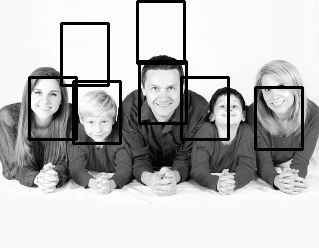
\includegraphics[width=\textwidth]{family_labeled_nms}
        \caption{Imagen tras aplicarla \textit{Non-Maximum supresion}}
         \label{subfig:family_labeled_nms}
    \end{subfigure}
        \caption{Resultados tras aplicar el clasificador sobre una imagen}
	\label{fig:5.1.4}
\end{figure}

\section{Conclusiones}

El método utilizado en esta sección se encuentra muy limitado por los siguientes aspectos:

\begin{itemize}
	\item Es una técnica que presenta problemas de rendimiento. Puesto que requiere de 2 o 3 segundos, como mínimo, para clasificar una nueva imagen.
	\item Es una técnica que no tiene en cuenta el contexto de la imagen para su clasificación. Sino, que solo tiene en cuenta cada uno de los fragmentos de la imagen de manera aislada al resto. Lo cual dificulta una adecuada precisión del clasificador.
	\item Comete muchos errores en la detección de falsos positivos. Como se puede observar en la figura \ref{subfig:family_labeled_nms}.
	\item El tamaño de la subdivisión de la imagen es constante. Por lo tanto, complica las posibilidades en la detección de distintos tamaños de fitolitos.
\end{itemize}

\section{Problema fundamental: falta de imágenes}

Llegados a este punto, y teniendo una primera aproximación, con mayor o menor precisión, de como afrontar el reconocimiento automático de fitolitos, se plantea un problema fundamental en el desarrollo de este proyecto. El problema, al que me refiero, es que no poseemos o conocemos ningún conjunto de entrenamiento de imágenes etiquetadas\footnote{Me refiero por imágenes etiquetadas, a imágenes con las coordenadas de donden se encuentran los distintos fitolitos en estas.} de fitolitos. Y por lo que hemos podido observar, hasta el momento, es el requisito básico en el aprendizaje supervisado.

Debido a esta problemática, desarrollamos un etiquetador de fitolitos que permita a nuestros usuarios crear un conjunto de imágenes de fitolitos etiquetadas y así, solucionar este problema fundamental en el desarrollo del proyecto.

En concreto, este etiquetador es una aplicación web desarrollada sobre un conjunto de tecnologías \textit{Python} y \textit{JavaScript}. Con el objetivo de poder realizar un futuro despliegue en un servicio \textit{web} que facilite lo máximo las tareas a nuestros usuarios. La información más detallada para un futuro programador, o para el uso por parte del usuario, se encuentra en los anexos del manual del programador y el manual del usuario, respectivamente.

\section{Detección de objetos mediante técnicas de \textit{deep learning}}

Una vez observados los resultados mediante una técnica clásica, como es \textit{sliding window}. Vamos a ir un paso más allá, con las técnicas de \textit{deep learning}, las cuales son las que,  con diferencia, mayor rendimiento aportan en la actualidad, como previamente he explicado en los conceptos teóricos.

Para ello, vamos a entrenar una implementación de \textit{YOLO} en \textit{Python}, todavía en desarrollo, para tratar de llevar a cabo el detector automático de fitolitos. Aunque, existen otras alternativas que se podrían adoptar en un fúturo de no conseguir los resultados esperados con esta implementación.

Previamente, en los conceptos teóricos, se ha explicado que este tipo de modelos también presentan algunas problemáticas, por el volumen de imágenes necesario y el tiempo necesario para ser entrenados, principalmente. Existen soluciones, como \textit{data augmentation}, trasferencia de conocimiento o partir de modelos previamente entrenados. Que iremos valorando en este desarrollo.